\documentclass[12pt,a4j]{jarticle}
\usepackage[dvipdfmx]{graphicx}
\usepackage{url}
\begin{document}
\title{コンピュータリテラシレポート#14}
\author{i2524002, 石田幸太}
\date{2025年7月23日}
\maketitle

\section{グループで決めたテーマ、グループ全員の名前と学籍番号、URL}

\subsection{テーマ}
テーマは「NetflixのWebサイト模倣」とした。理由は、普段使用しているプラットフォームのデザインや機能を自分たちで再現することで、Web制作の実践的なスキルを身につけることができると考えたためである。また、これまでの授業を通して培った知識や技術力を元に、既に使われているサービスのwebサイトを作れるのかどうかを試すためでもある。

\subsection{グループ全員の名前と学籍番号}

\begin{description}
\item[i2524002] 石田幸太(トップページ・トップページ英語・全体のデザイン(css)担当)
\item[f2524023] 深堀友翔(サインアップページ・サインアップページ英語・サインインページ・サインインページ英語担当)
\end{description}

\subsection{完成したサイトの URL}

\url{http://www.edu.cc.uec.ac.jp/~i2524002/Netflix-Cloning/index.html}


\section{グループ作業 (コンセプト、デザイン、設計) の内容}

\subsection{コンセプト}
普段使用しているプラットフォームのWebサイトを自分たちで再現することを目標とした。
意図としては、実際に使えるクオリティのものを作れるのかどうかの試行である。
Netflixを選んだ理由は、単純にチームメンバー全員がよく使うサービスであるからである。

\subsection{デザイン}
全体の配色やレイアウトはNetflix本家を参考にしつつ、グループ内で意見を出し合い、トップページとサインイン・サインアップページで統一感を持たせることを重視した。黒を基調とした配色に、Netflixの象徴的な赤色をアクセントカラーとして使用した。CSSは石田(私)が中心となって作成し、全ページで共通のスタイルを適用することで、デザインの一貫性を保った。

\subsection{設計}
サイト構成は以下のように設計した。
\begin{itemize}
\item 入口ページ(トップページ):日本語・英語の2言語対応
\item サインインページ:日本語・英語の2言語対応
\item サインアップページ:日本語・英語の2言語対応
\end{itemize}

当初は各コンテンツの詳細ページ(映画やドラマの紹介ページなど)も作成することを検討したが、素材収集や複雑なレイアウト実装に時間がかかりそうだったため、今回は基本的なページ構成に絞って制作することとした。

ページごとに担当を分担し、石田がトップページ(日本語・英語)および全体のデザイン、深堀がサインイン・サインアップページ(日本語・英語)を担当した。各ページの内容や構成は事前にメモで設計し、グループ内で確認・調整を行った。

\section{自分が担当したページの報告}
私はトップページ(日本語・英語)および全体のデザイン(CSS)を担当した。

\subsection{トップページ(日本語)}
Netflixの本家トップページを参考に、以下の要素を重視して制作した。
\begin{itemize}
\item ヒーローイメージとキャッチコピーの配置
\item 「今すぐ始める」ボタンの目立つ配置
\item サービスの特徴を紹介するセクションの構成
\item レスポンシブデザインを意識したレイアウト
\end{itemize}

特に工夫した点は、JavaScriptを使用して画像やボタンのホバー効果を追加し、ユーザーが直感的に操作できるようにしたことである。また、レスポンシブ対応されたレイアウトになるよう、CSSのメディアクエリを活用した。

\begin{figure}[htbp]
\begin{center}
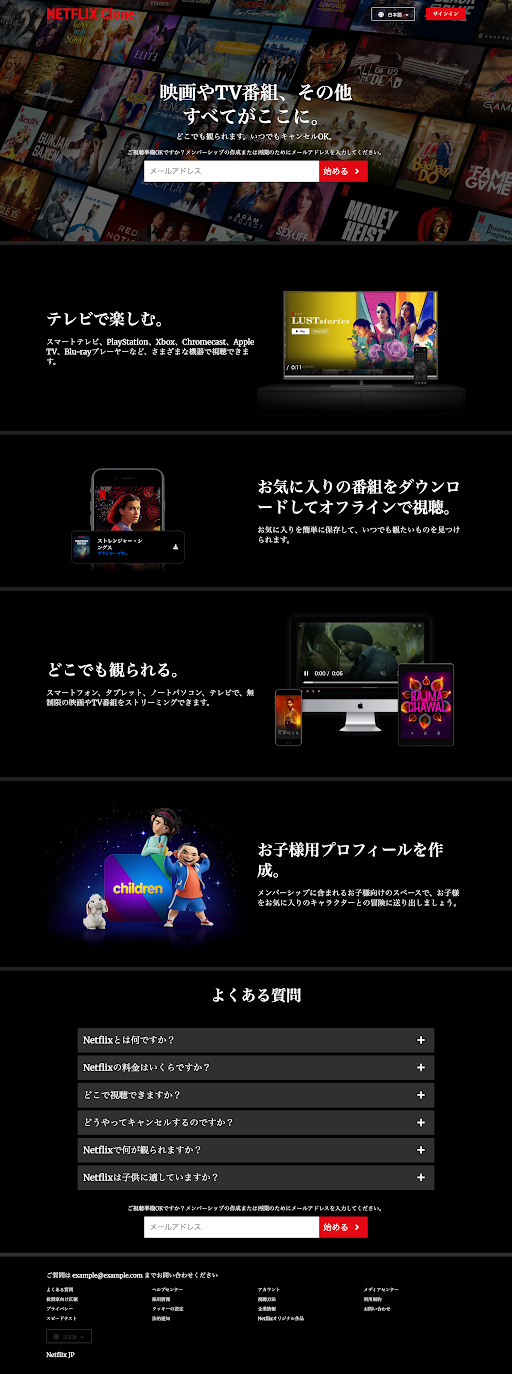
\includegraphics[width=12cm]{top.png}
\caption{トップページ(日本語)の表示例}\label{fig1}
\end{center}
\end{figure}

\subsection{トップページ(英語)}
日本語ページと同じ構成で、テキスト部分のみ英語に差し替えて制作した。多言語対応のため、HTMLファイルを分けて管理し、言語切り替えのリンクも設置した。英語版では、文字数の違いによるレイアウトの崩れがないよう、CSSの調整も行った。

\begin{figure}[htbp]
\begin{center}
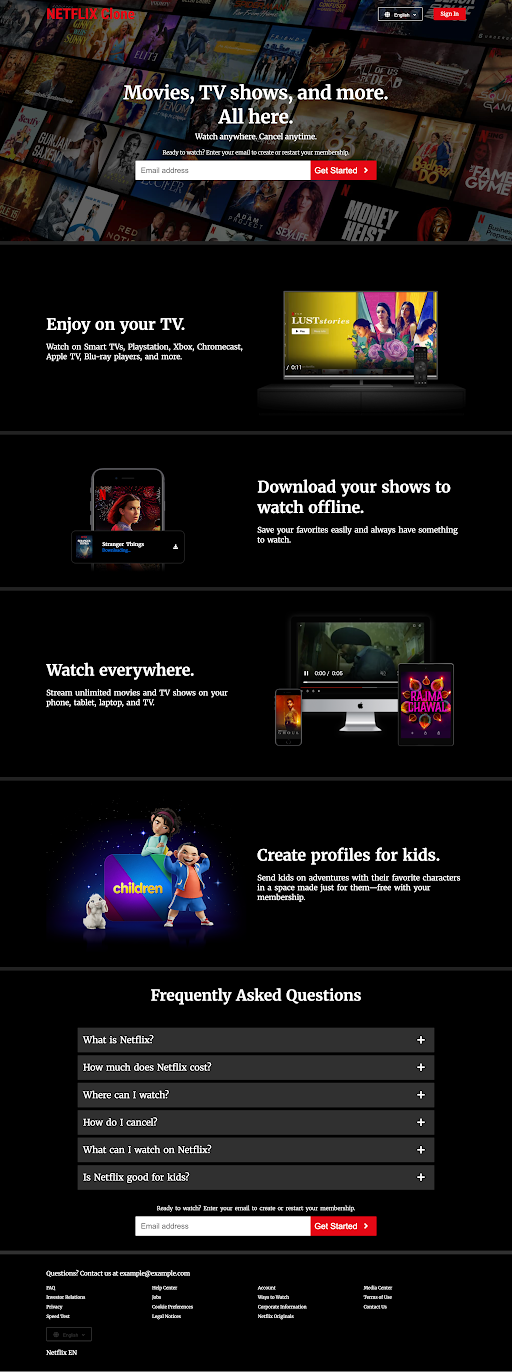
\includegraphics[width=12cm]{top_en.png}
\caption{トップページ(英語)の表示例}\label{fig2}
\end{center}
\end{figure}

\subsection{全体デザイン(CSS)}
サインイン・サインアップページも含め、全体の配色・フォント・ボタンデザインを統一した。具体的には以下のようなものを設定した。
\begin{itemize}
\item 配色:黒を基調とし、Netflixの赤色をアクセントに使用
\item フォント:可読性を重視したサンセリフ系フォントを選択
\item ボタン:統一されたデザインとホバー効果を実装
\item レイアウト:すべてのページで一貫したマージンとパディングを設定
\end{itemize}

グループ内で意見を出し合い、シンプルで見やすく、かつNetflixらしいデザインを目指した。
また、デザインの統一性を保つために、CSSのメディアクエリを活用した。

\begin{figure}[htbp]
\begin{center}
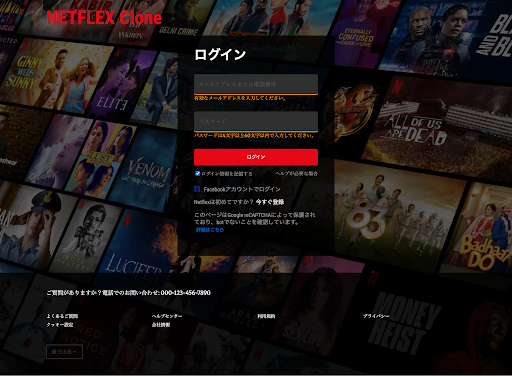
\includegraphics[width=10cm]{login.png}
\caption{サインインページ(日本語)の表示例}\label{fig3}
\end{center}
\end{figure}

\begin{figure}[htbp]
\begin{center}
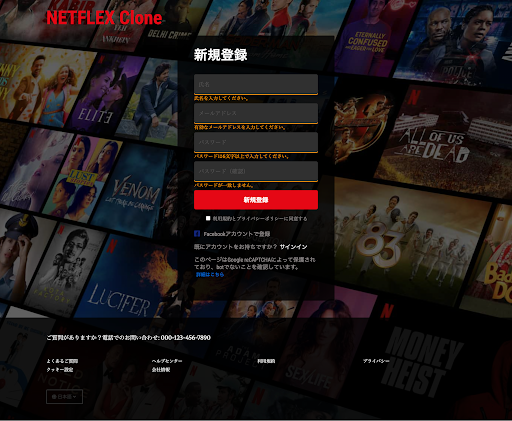
\includegraphics[width=10cm]{sign_up.png}
\caption{サインアップページ(日本語)の表示例}\label{fig4}
\end{center}
\end{figure}

\section{考察}
今回の課題を通じて、実際のサービスを模倣することでWeb制作の実践的なスキルが大幅に向上した。特に以下の点で学びが多かった。

\begin{itemize}
\item CSSによるレイアウト調整
\item メディアクエリを活用したレスポンシブデザインの実装方法
\item グループでの役割分担と協力の重要性
\item デザインの統一性を保つためのコミュニケーション
\end{itemize}

今回は特に、完成度を統一するための他者とのコミュニケーションについて学ぶことが多かった。グループでWebサイトを制作する際は、各メンバーの技術レベルや作業スタイルが異なるため、品質のばらつきが生じやすい。しかし、継続的な情報共有と相互チェックを行うことで、全体の品質を一定に保つことができることを実感した。
今回は私がリーダー的役割となり、レビューをさせていただいた。エンジニア業務の実務を体感したような体験だった。

\section{アンケート}

\subsection{Q1:Webサイトをグループで協力して製作してみて、どのようなことが分かりましたか。}
一人では思いつかないアイデアや改善点を他のメンバーから得ることができ、より質の高いWebサイトを制作することができた。
ここで言う「質の高い」というのは、クオリティ面ではなく"より本質的な学習"のことも指している。
特に、事前の設計と継続的なコミュニケーションが重要であることを実感した。(余談だが、AI活用も最初の設計が大事であり、それは人間かAIか問わないと再認識した)

\subsection{Q2:今回のようなレポートは何がよかったですか。何が大変でしたか。}
良かった点は、授業で学んだ技術を他チームメイトと一緒に話し合いながら一つのプロダクトを作ることができたこと。
大変だった点は、グループメンバーの技術レベルや作業スタイルが異なるため、品質のばらつきが生じやすいこと。
また、グループメンバーの作業スタイルが異なるため、進捗管理が難しいことも大変だった点として挙げられる。

\subsection{Q3:リフレクション (今回の課題で分かったこと)・感想・要望をどうぞ。}
実際のサービスを模倣することで、Web制作の流れや注意すべきポイントを実感できた。特に、ユーザーの視点に立ったデザイン実装のために細かく内外余白が調整されていたり、技術的な制約の中でいかに理想的なデザインを実現するかの難しさを学んだ。今後はJavaScriptやライブラリを使用したより動的な機能の実装や、アクセシビリティを考慮したWebサイト制作にも挑戦したい。

\end{document}